\graphicspath{{img/appendix}{img/impl}}

\newcommand\invisiblesection[1]{%
  \refstepcounter{chapter}%
  \addcontentsline{toc}{chapter}{\protect\numberline{\thechapter}#1}%
  \sectionmark{#1}}

\invisiblesection{Hyperparameter Optimization}
\clearpage
\subsubsection{Hyperparameter Optimization Plots (moving avg. of 8)}
\label{app:hyperparam_optim}
\begin{figure}[H]
    \advance\leftskip-2.3cm
    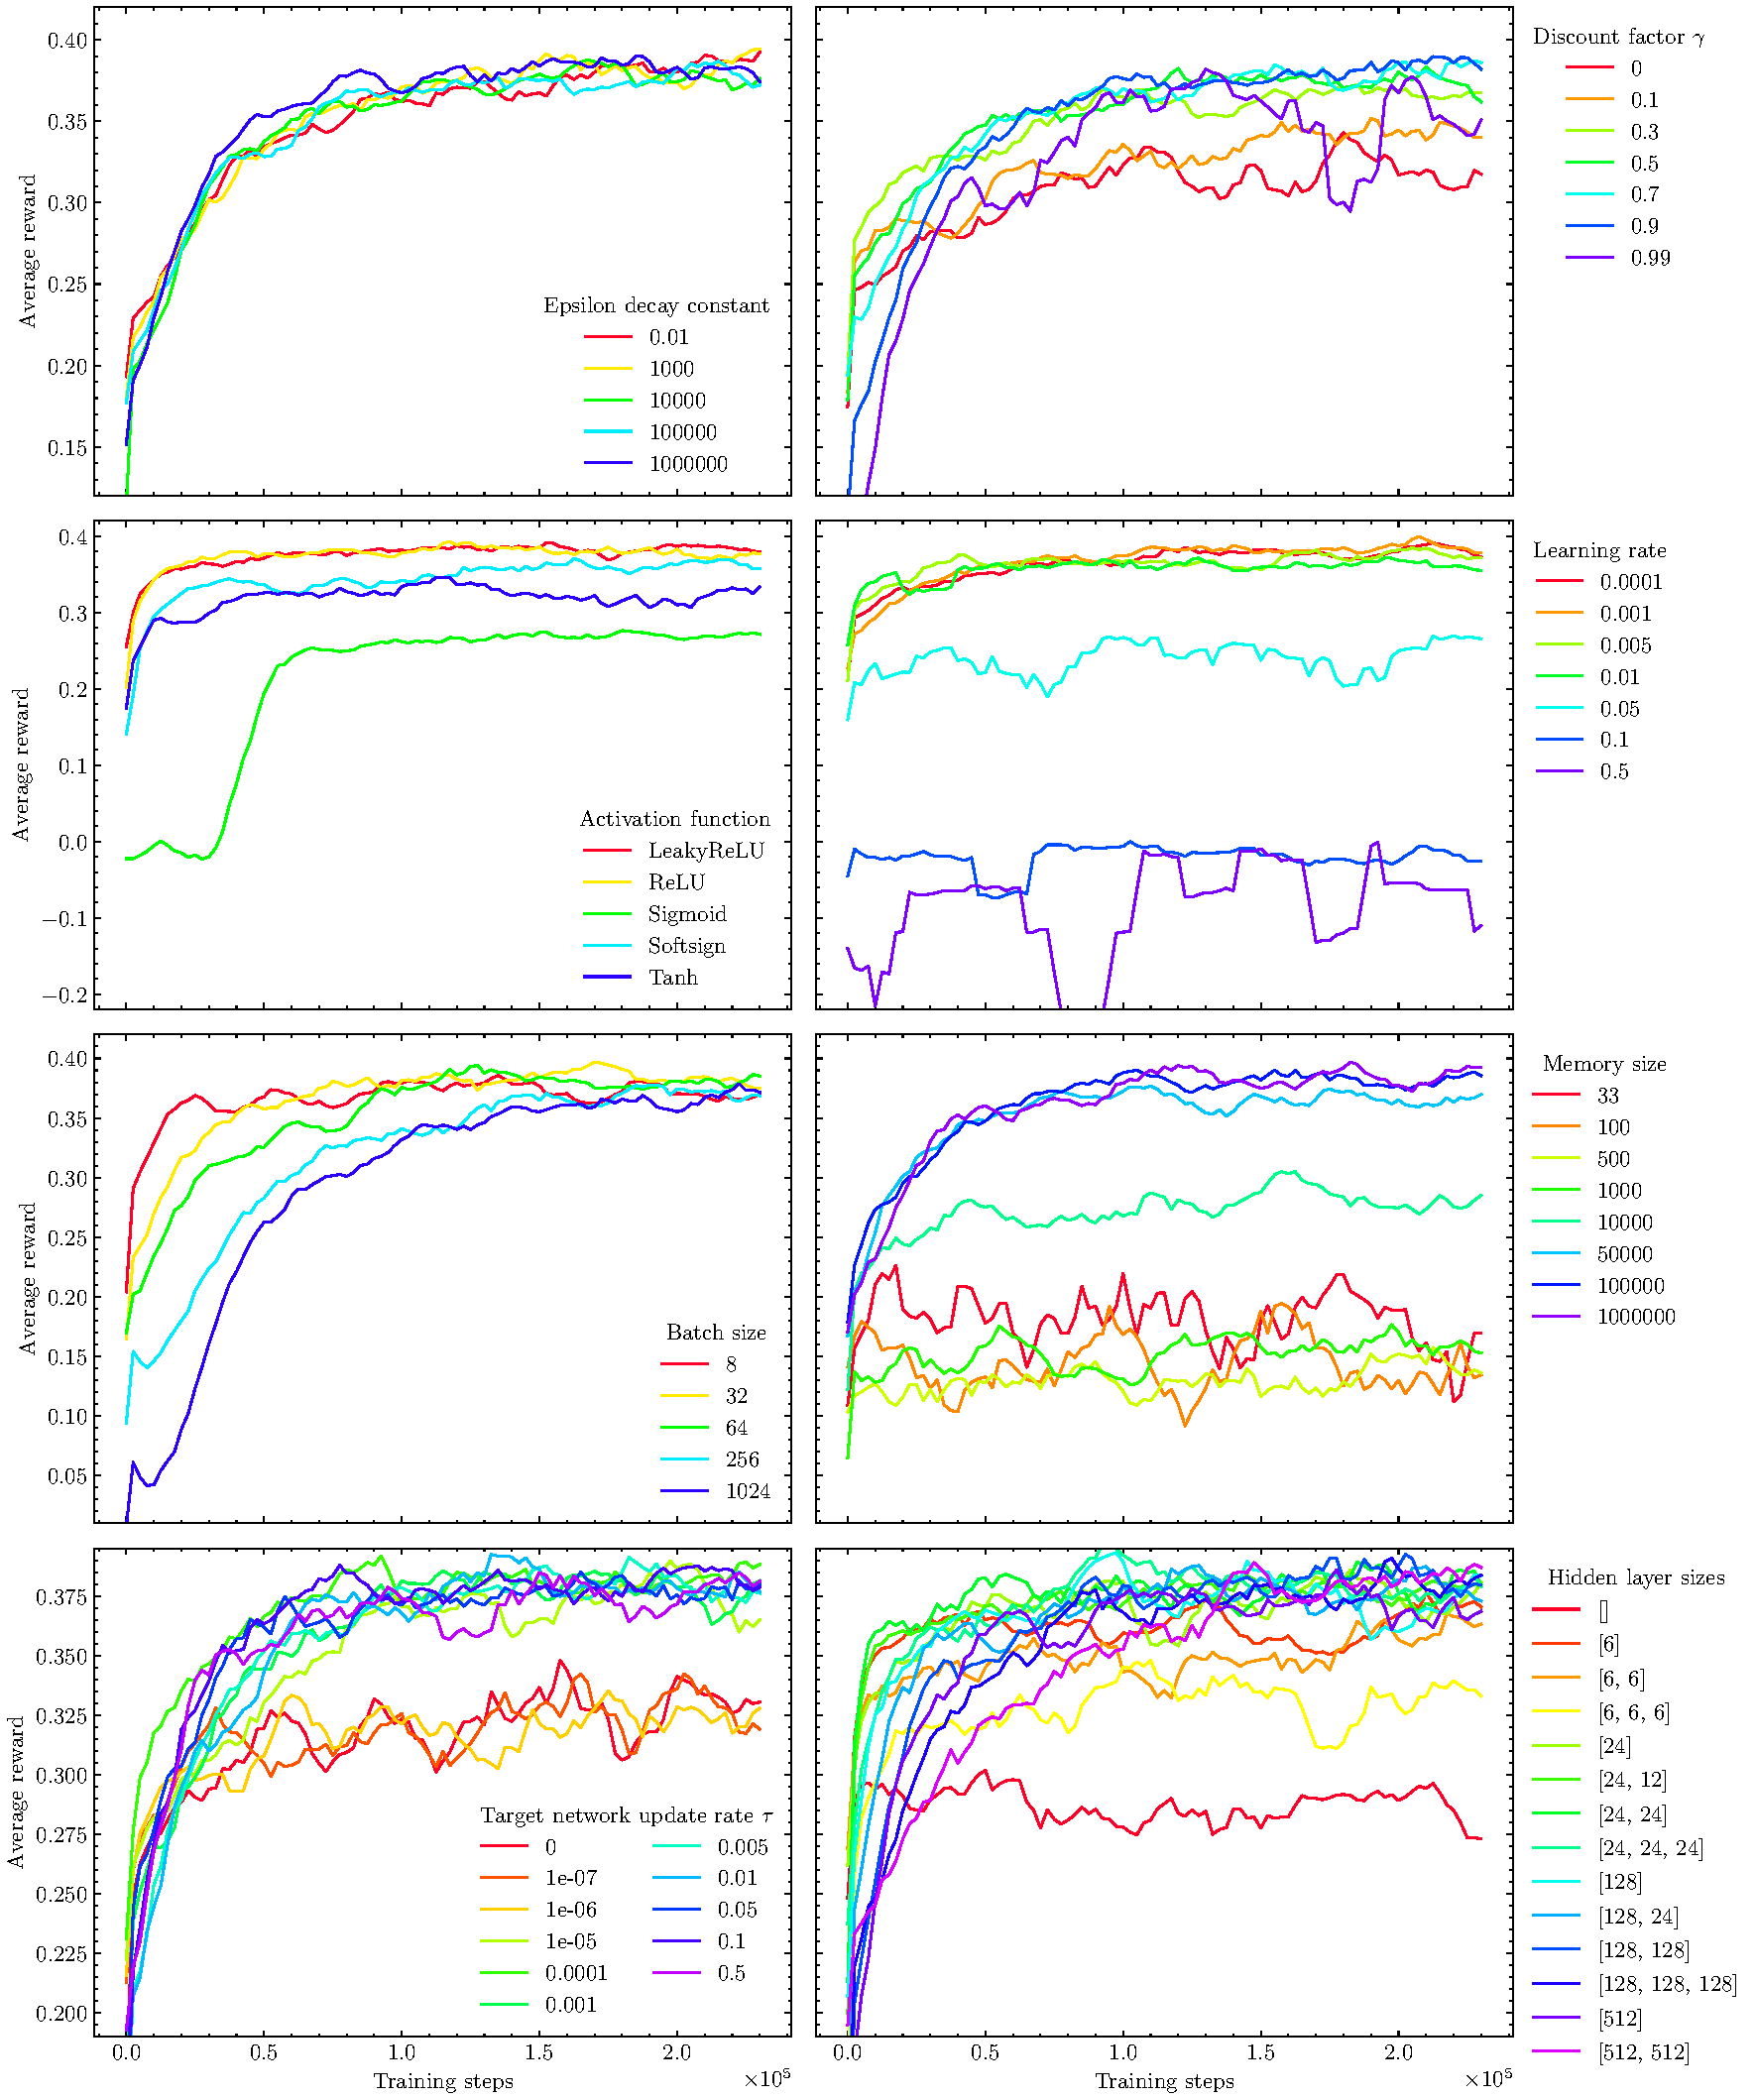
\includegraphics[width=1.28\textwidth]{hyperparam_optim_8_sci.pdf}
    \caption{Hyperparameter optimization plots analyzed in section \ref{sec:hyperparam_optim}.}
    \label{fig:hyperparam_optim_8}
\end{figure}

\subsubsection{Hyperparameter Optimization Plots (moving avg. of 30)}
\label{app:hyperparam_optim_30}
\begin{figure}[H]
    \advance\leftskip-2.3cm
    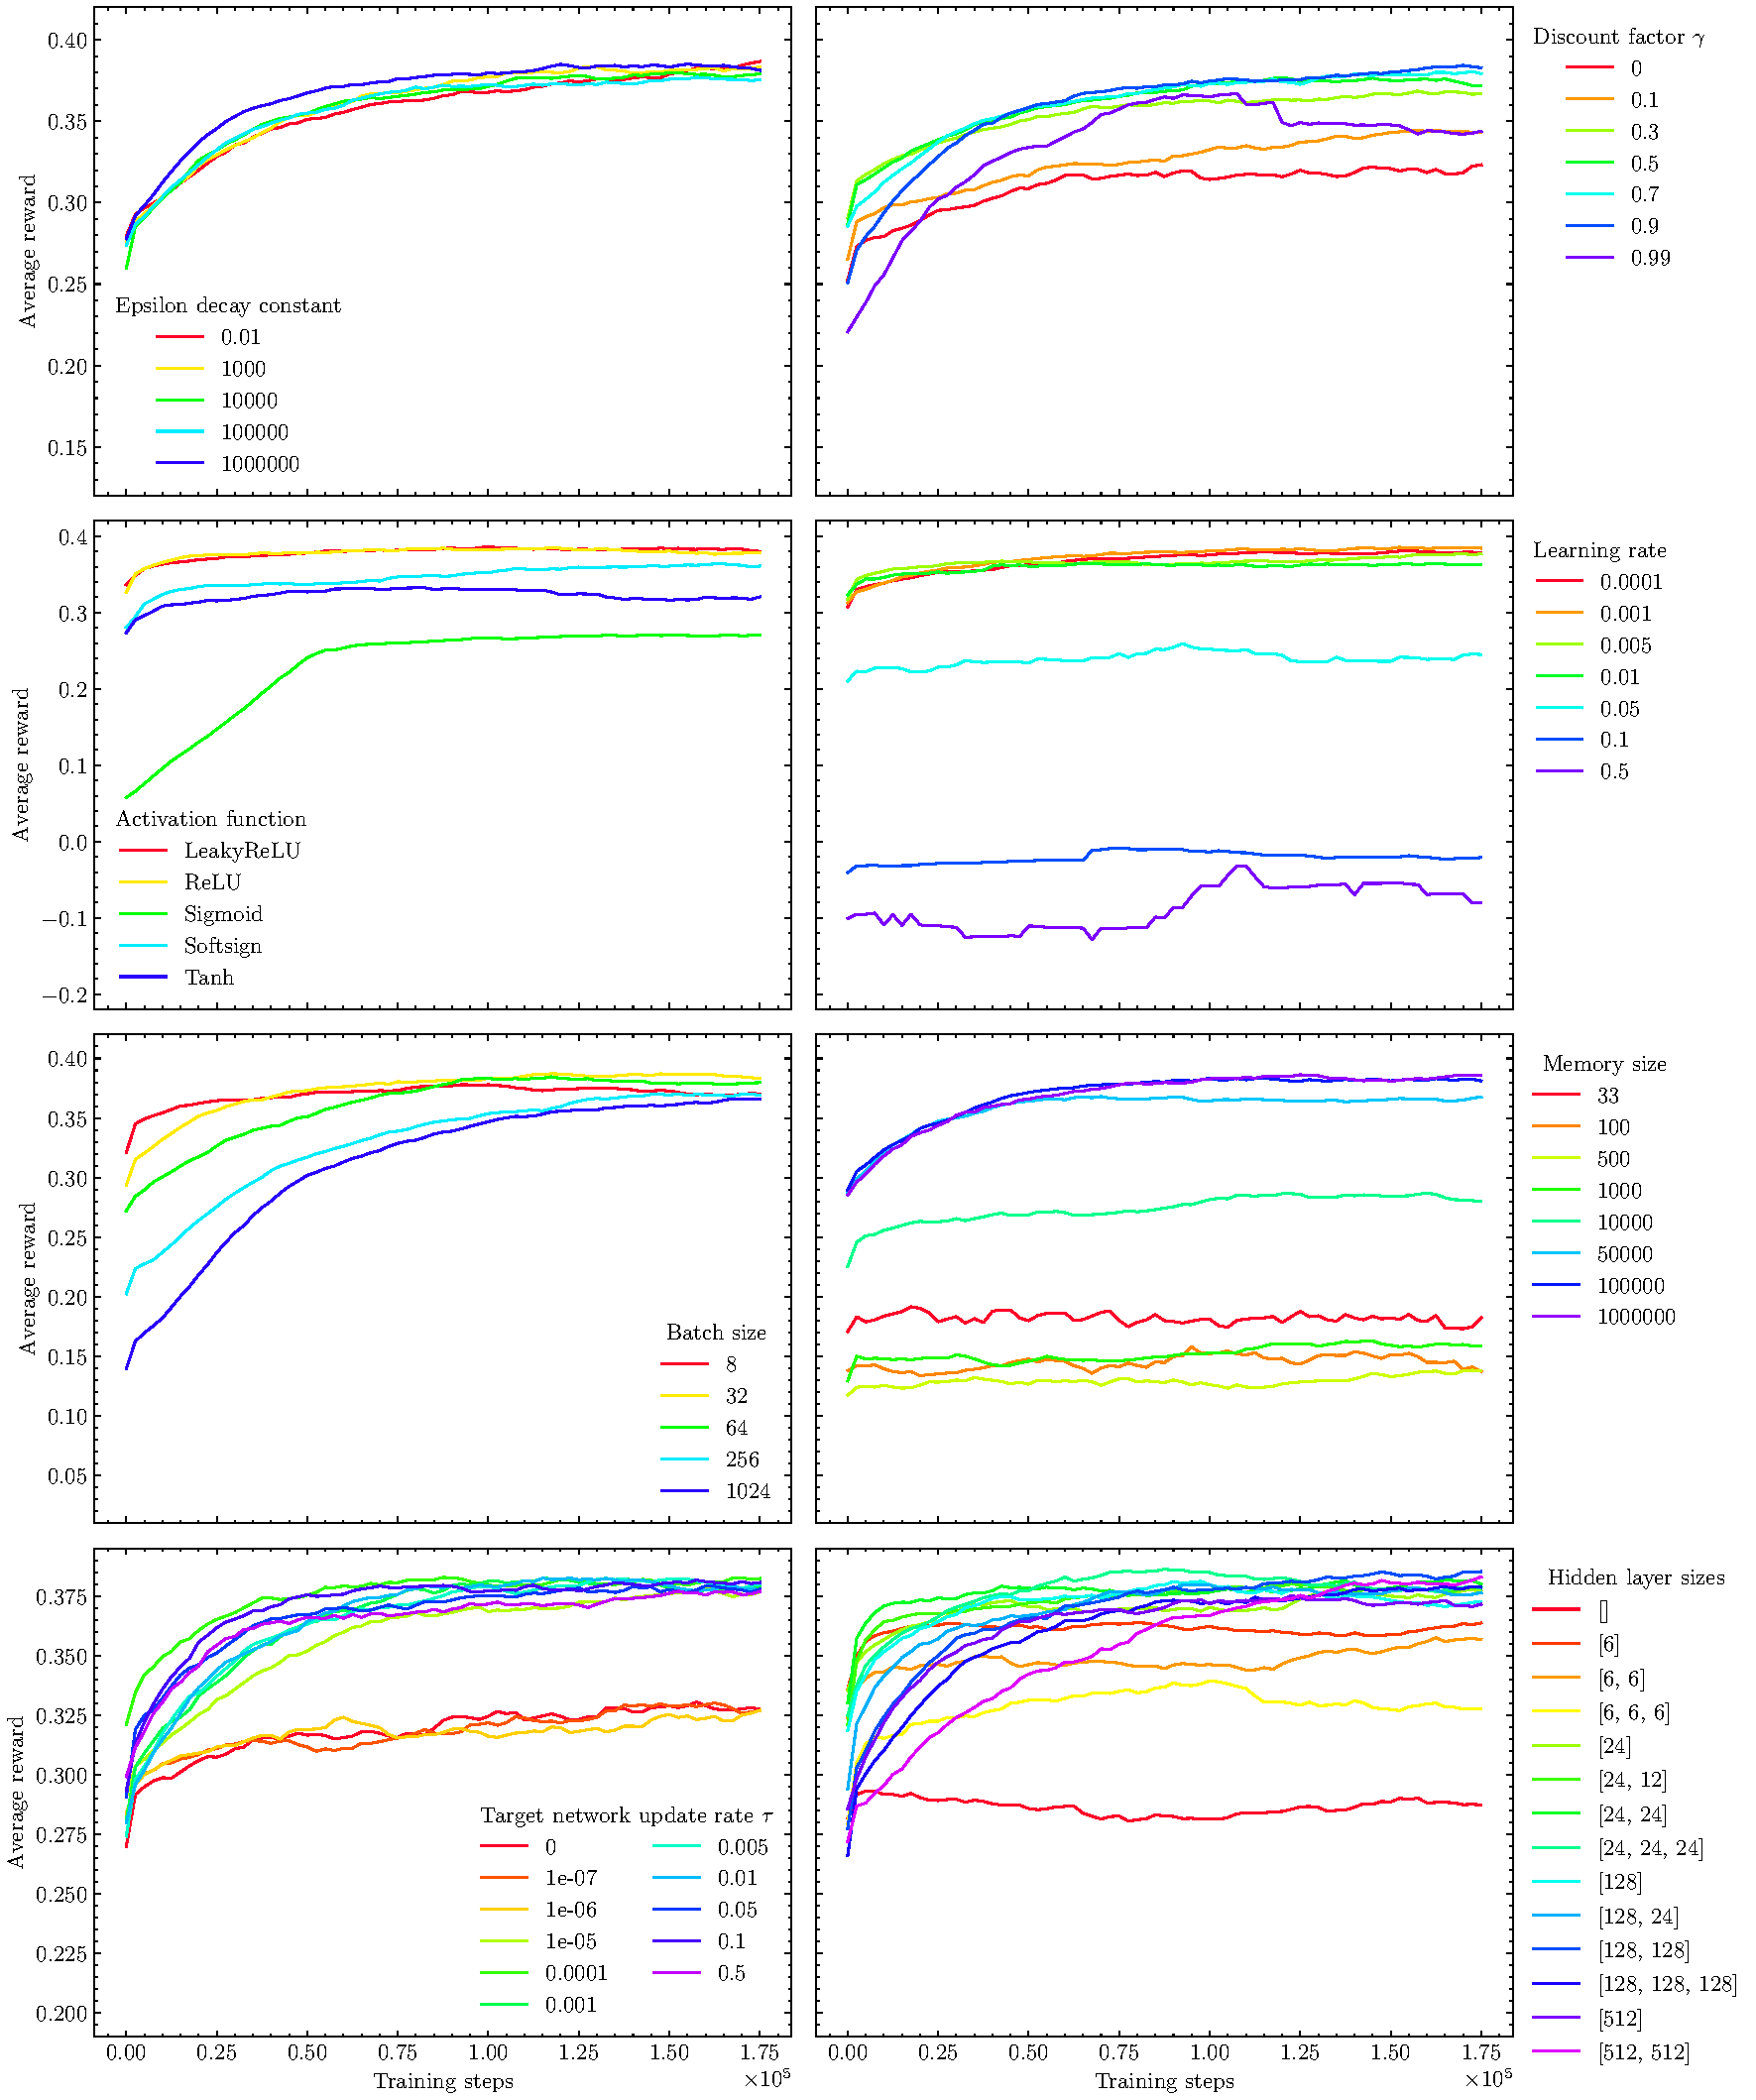
\includegraphics[width=1.28\textwidth]{hyperparam_optim_30_sci.pdf}
    \caption{Hyperparameter optimization plots analyzed in section \ref{sec:hyperparam_optim}.}
    \label{fig:hyperparam_optim_30}
\end{figure}


\chapter{Code}
\label{app:code}
only for reproducibility
rest of code is on github, packasge easy to use
setup like this
\section{First training}
